For submodular value of information estimation functions, the myopic algorithm 
is nearly optimal \cite{Guestrin.submodular}. Frequently, however, VOI estimates
are not submodular, and no non-trivial performance guarantees can be provided.
The simplifying assumptions behind the myopic estimate  are related
to the notion of {\it non-increasing returns}: an implicit hypothesis that the intrinsic
value of information grows slower than the cost. When the hypothesis is correct,
the assumptions should work well; otherwise, the myopic algorithm either
gets stuck or makes measurements which gain little useful information.

\begin{figure}[h]
\centering
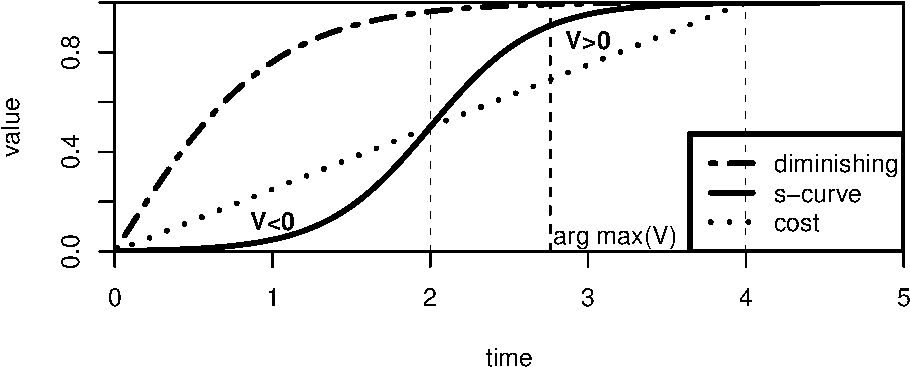
\includegraphics[scale=0.48]{s-curve.pdf}
\caption{Value of information curves} 
\label{fig:greedy-s-curve}
\end{figure} 

The {\it law of diminishing returns} \cite{Johns.economics}
only holds asymptotically: while it is often true that starting at
some point in time the returns never grow, until that point they can
alternate between increases and decreases. Figure~\ref{fig:greedy-s-curve}
shows a curve of diminishing returns (the
dashed curve), an s-curve (the solid curve), and the areas with
negative and positive values for the s-curved returns for a linear
time cost (the dotted straight line). Investments for the first two units
of time do not pay off, and the maximum return is achieved at
approximately $2.8$.

Sigmoid-shaped returns were discovered in marketing
\cite{Johansson.s-curve}.  As experimental results show
\cite{Zilberstein.sensing}, they are not uncommon in sensing and
planning. In such cases, an approach that can deal with increasing
returns must be used.

Even in simple cases the myopic estimate may behave poorly.  Consider
the following example:
\begin {itemize}
\item $S$ is a set of two items $s_1$, $s_2$ with a single feature $z$; 
\item the value of feature $z$ for $s_1$ is known exactly, $z(s_1)=1$;
\item the initial belief about $s_2$ is a normal distribution $P_0(z(s_1))=\mathcal{N}(0,1)$;
\item the observation distribution is a normal distribution, $P^m(z^m|z)=\mathcal{N}(z, 5)$;
\item the measurement cost is constant, and chosen so that the net
  value estimate of a two-observation step is zero: $c^m=\frac {MVI_2^2} 2\approx
  0.00144$; the movement cost is zero.
\item the utility is a step function:
\[u(x) = \left\{ 
\begin{array}{l l}
  0 & \quad \mbox{if $x<1$}\\
  0.5 & \quad \mbox{if $x=1$}\\
  1 & \quad \mbox{if $x>1$}\\
\end{array} \right.
 \]
\end {itemize}

The plot in Figure~\ref{fig:greedy-mvilim-value-cost} depicts the intrinsic
value of information as a function of the number of measurements in a single
step. The straight line corresponds to the measurement cost.

\begin{figure}[h]
\centering
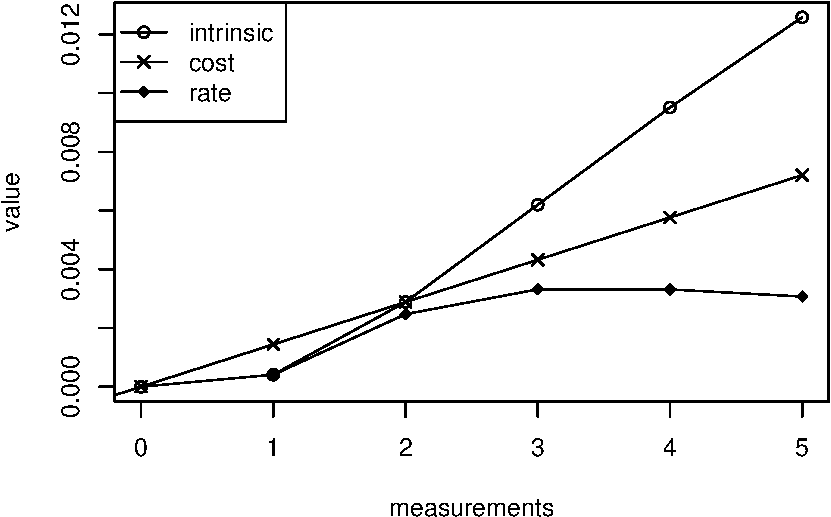
\includegraphics[scale=0.48]{mvilim-value-cost.pdf}
\caption{Intrinsic value and measurement cost} 
\label{fig:greedy-mvilim-value-cost}
\end{figure} 

Under these conditions, the pure myopic algorithm (which considers
only one measurement per step)
will terminate without gathering evidence because the value estimate
of the first step is negative, and will return item $s_1$ as
best. However, observing $s_2$ several times in a row has a positive
value, and the updated expected utility of $s_2$ can eventually become
greater than $u(z(s_1))$.  Figure~\ref{fig:greedy-mvilim-value-cost} also
shows the intrinsic value growth rate as a function of the number of
measurements: the rate increases up to a maximum at 3 measurements,
and then goes down. Apparently, the myopic algorithm does not ``see''
as far as the initial increase.

As the pure myopic scheme is too short-sighted in many cases,
some lookahead is needed, at increased computational cost.
The proposed semi-myopic optimization framework enables
a spectrum of schemes that allow a choice of such tradeoffs.
The scheme is analyzed qualitatively,
and theoretical bounds for two important extreme cases are presented.

Keeping the complexity manageable while
overcoming the limitations of the myopic algorithm
is the basis for the {\em semi-myopic} framework.
One might consider finding an optimal measurement policy, but
the number of possible measurement plans,
even for discrete variables, is super-exponential
(and uncountably infinite for continuous variables), which 
makes this approach infeasible.
In the semi-myopic schemes we essentially assume (only for the sake of
estimating VOI), that we need to select
measurements offline, without observing the results of previous
observations. This makes the (simplified, but incomplete) search space ``only''
exponential in the general case, and polynomial in important,
useful special cases.

Let ${\mathcal M}$ be the set of all possible measurement
actions, and ${\mathcal C}$ be a constraint over sets of
measurements from ${\mathcal M}$. In the semi-myopic framework,
all possible subsets (batches) ${\mathcal B}$ of measurements from ${\mathcal M}$
that obey constraint ${\mathcal C}$ are considered: for each
such subset ${\mathcal B}$ a `batch' value of information estimate is computed
under the assumption that all measurements in ${\mathcal B}$ are made, 
followed by
a decision (selection of an item). Then, the batch
${\mathcal B}^*$ with the best value estimate is chosen. Once 
${\mathcal B}^*$ is chosen, there are still several options
(\cite{BilgicGetoor.voila} discusses a similar approach to discrete
feature acquisition):
\begin{enumerate}
\item Actually do all the measurements in ${\mathcal B}^*$.
\item Attempt to optimize ${\mathcal B}^*$ into some form of
  conditional plan of measurements.
\item Perform (for now) only the best measurement in ${\mathcal B}^*$.
\end{enumerate}

In all cases, after measurements are made, the selection of measurements is repeated,
until no batch has a positive value, at which point the algorithm {\em
  terminates} and selects an item. Option 1, a combination of online
and offline selection, misses the possibility to choose better
measurements while executing a batch, and therefore is inferior to
options 2 and 3. While limited efficient implementation for option 2 is
possible, optimizing a conditional plan is intractable in general,
recreating the optimal policy problem on a smaller scale.  
Option 3, allows better use of information from
the outcome of previous measurements, and remains tractable.

% In the semi-myopic version, the measurement selection part
% (lines~\ref{alg:greedy-select-start}--\ref{alg:greedy-select-end})
% of the algorithm in Figure~\ref{alg:greedy-algorithm} is
% replaced with the algorithm in Figure~\ref{alg:semi-myopic-scheme}.

The semi-myopic version of the greedy algorithm is presented in
Figure~\ref{alg:semi-myopic-scheme}. 
\begin{figure}
\begin{algorithmic}[1]
\STATE $budget \leftarrow C$
\STATE Initialize joint distribution $P$ to $P_0$ \label{alg:semi-myopic-initialize-beliefs}
\LOOP                        \label{alg:semi-myopic-main-loop-start}
  \STATE {\bf for all} items $s_i$ {\bf do} Compute $\IE_P(U_i)$ \label{alg:semi-myopic-compute-eu}
  \FORALL {batches $b_j$ satisfying constraint $\mathcal{C}$}  \label{alg:semi-myopic-select-start}\label{alg:semi-myopic-compute-batch-start}
    \IF {$cost(b_j) \ge budget$}
      \STATE Compute $V_j^b$
    \ELSE
      \STATE $V_j^b \leftarrow 0$ \label{alg:semi-myopic-batch}
    \ENDIF
  \ENDFOR                         \label{alg:semi-myopic-compute-batch-end}
  \STATE $j_{max} \leftarrow \arg \max\limits_j V_j^b$
  \IF {$V_{j_{max}}^b>0$}
    \STATE {\bf for all} {measurements $m_k \in b_{j_{max}}$} {\bf do} Compute $V_k$  \label{alg:semi-myopic-voi}
    \STATE $k_{max} \leftarrow \arg \max\limits_k V_k$
    \STATE Perform measurement $m_{k_{max}}$ \label{alg:semi-myopic-measure}
    \STATE Update joint distribution $P$ \label{alg:semi-myopic-update-beliefs}
    \STATE $budget \leftarrow budget-c_{k_{max}}$  \label{alg:semi-myopic-select-end}
  \ENDIF
  \STATE {\bf else break} \label{alg:semi-myopic-break}
\ENDLOOP                \label{alg:semi-myopic-main-loop-end}
\STATE $\alpha \leftarrow \arg \max \IE_P(U_i)$ \label{alg:semi-myopic-return-alpha}
\RETURN $s_\alpha$
\end{algorithmic}
\caption{Semi-myopic Scheme}
\label{alg:semi-myopic-scheme}
\end{figure}
The value of information is computed twice: first, value of
information $V_j^b$ of every batch $b_j$ satisfying the constraint
$\mathcal{C}$ is computed (line~\ref{alg:semi-myopic-batch});
then, if the maximum value of information of a batch is positive,
value of information $V_k$ of every single measurement $m_k$ from
the batch $b_{j_{max}}$ is computed
(line~\ref{alg:semi-myopic-voi}), and a measurement with the highest
net value of information (even if negative) is performed.

The meta-reasoning approach (Section \ref{sec:bg-limited}) requires
that computation time be small compared to the measurement
time. Assuming that the value of information of a set of measurements 
and the expected utility of an item can be computed in constant times
$T_V$ and $T_{EU}$ respectively, the computation time  $T_{comp}$ of a single
step of the algorithm is the sum of:

\begin{itemize}
\item the time $T_{eu}$ to compute utilities of all items
  (line~\ref{alg:semi-myopic-compute-eu}),
  $T_{eu}=O(T_UN_s)$;
\item the time $T_{batch}$ to compute values of information of all batches
  according the constraint $\mathcal{C}$
  (lines~\ref{alg:semi-myopic-select-start}--\ref{alg:semi-myopic-select-end}),
  $O(T_V|\mathcal{C}(N_s, N_m)|)$;
\item the time $T_{voi}$ to compute values of information of every single
  measurement in the best batch
  (line~\ref{alg:semi-myopic-voi}),
  $O(T_VN_sN_M)$ --- a single batch may contain all types of
  measurements for each of the items;
\item Assuming the time $T_{bel}$ to update the joint distribution
  (line~\ref{alg:semi-myopic-update-beliefs}) is constant and
  sufficiently small (using approximate inference
  algorithms), denote $T_{bel}$ by $T_B$.
\end{itemize}
\begin{equation}
  \label{eq:thr-computation-time}
  \hspace{-8em}T_{comp}=T_{eu}+T_{batch}+T_{voi}+T_{bel}
\end{equation}
\vspace{-2em}
\begin{equation*}
\hspace{2em}=O(T_UN_s)+O(T_V|\mathcal{C}(N_s, N_m)|)+O(T_VN_sN_M)+T_B\nonumber
\end{equation*}

$T_{batch}$ is the greatest term in $T_{comp}$ and determines the
computational time complexity of the algorithm according to a
semimyopic {\em scheme} defined by the constraint $\mathcal{C}$.  For
the empty constraint --- the {\em exhaustive} scheme --- all possible
measurement sets are considered; this scheme has an exponential
computation time, while {\em still} not guaranteeing optimality (finding an
\emph{optimal} solution requires examination of all \emph{conditional plans}).
Nevertheless, this scheme is a good yardstick against which
to compare other semi-myopic schemes, as done in Section \ref{sec:emp},
as it is unreasonable to expect {\em any} semi-myopic scheme to
achieve a result better than the exhaustive scheme in terms of the objective
function (costs of measurements and utility of selected item).

At the other extreme is the constraint where only singleton
sets are allowed. This extreme results in the greedy single-step
assumption --- the original myopic scheme, which is the
current state of the art for the general selection problem.
\cite{BilgicGetoor.voila} proposes a constraint based 
on the {\em value of information lattice},
a data structure introduced in that paper. The induced number of
subsets is still exponential in a general case, but for certain kinds
of dependency structure the constraint gives significant
improvement. Yet another---{\em omni-myopic}---constraint can be
constructed along the lines of \cite{Heckerman.nonmyopic}: the
measurements are ordered according to their myopic VOI estimates, and
subsets of measurements with greatest VOI estimates are considered.

This paper suggests the constraint that restricts batches to
repeated identical measurements---the {\em blinkered} scheme. This
scheme is tractable, corresponds to a common approach in which noisy
experiments are repeated to increase confidence, and demonstrates
improved efficiency in empirical evaluations.

\subsection{Blinkered Estimate}
\label{sec:thr-blinkered-estimate}

As stated above, the blinkered scheme considers sets of independent identical
measurements; this constitutes unlimited lookahead, but along a single
``direction'', as if one ``had one's blinkers on''.  Although this
scheme has a computational overhead over the myopic one, the factor is
only linear in the budget. \footnote{Assuming either
  normal distributions, or some other distribution 
  where measurement and belief updating can be done, or at least
  approximated, efficiently.
  For general distributions, sets of observations may
  provide information beyond the mean and variance, and the resources
  required to compute value of information may even be exponential in
  the number of measurements.}  The ``blinkered'' value of information
is defined as:
\begin{eqnarray}
\label{eq:thr-bvi}
BVI_j\hspace{-0.8em}&=&\hspace{-0.8em}\max_n MVI_j^n\\
\mathrm{s.t.:\;}c_j\hspace{-0.8em}&=&\hspace{-0.8em}d(s_{last}, s_{i_j})+d(s_{i_j}, s_{i_j})(n-1)+c^m_{k_j}\leq C\nonumber
\end{eqnarray} 
where, as before, the $j$th measurement is of the $k_j$th type and
measures the $i_j$th item, $c_j$ is the net measurement cost, and
$s_{last}$ is the last measured item. 

Driven by this estimate, the blinkered scheme selects a single
measurement of the item where {\em some} number of measurements gains
the greatest value of information.  A single step is expected to be
just the first one in the right direction, rather than to actually
achieve the value. Thus, the estimate relaxes the {\it single-step}
assumption, while still underestimating the value of information.

For the blinkered scheme, $T_{batch}$ depends on the time
$T_{BVI}$ to compute the blinkered estimate for measuring an item:
\begin{equation}
\label{eq:thr-time-batch-blinkered}
T_{batch}=O(N_sN_mT_{BVI})
\end{equation}
For budget $C$ and a single measurement cost bounded from below
 by $c$, the time to compute the estimate $T_{BVI}$ is:
$T_{BVI}=O\left(T_{MVI}\frac C c\right)$.  This time bound (linear in the budget)
%still
%exponential in the representation 
is prohibitive for large budgets; but can be decreased in one of
the following ways:

\begin{itemize}
\item If $MVI^n$ is a unimodal function of $n$, which can be shown for some
  forms of distributions and utility functions,
  the time is logarithmic in the budget $C$. Indeed, using the
  bisection method to find $n$ for which $MVI^{n+1}-MVI^n$ changes sign
  yields the logarithmic time. $MVI^n$ is unimodal when, for example,
  the intrinsic value of information is represented by a translated S-curve
  shaped function of $n$, such as the logistic function or the sigmoid
  function, and the measurement cost is linearly proportional to
  $n$. S-curves are frequently met in learning \cite{Russell.aima},
  mathematical modeling \cite{Gershenfeld.modeling} and economics
  \cite{Johansson.s-curve}. $\Lambda(n)$ in the example in
  Section~\ref{sec:greedy-mvi-shortcomings} has the shape of an S-curve, and $MVI^n$
   is unimodal. 
\item $BVI$ can be computed for a bounded horizon $H$, such that
  $T_{BVI}=O\left(T_{MVI} \frac {\min (C, H)} c\right)$, and the
  choice of $H$ determines tradeoff between the measurement selection
  quality and the computation time.
\item $BVI$ can be estimated as the maximum for powers of
  2, $n=2^{n'}$: instead of selecting the maximum VOI for batches of
  1, 2, 3,~\ldots measurements, batches of 1, 2, 4, 8, 16,~\ldots
  measurements are considered.  This approach has been taken  in the implementation of
  the blinkered scheme used for the empirical evaluation (Section
  \ref{sec:emp}). Although $BVI$ is underestimated, the results of
  the blinkered scheme are still much better than of the myopic
  scheme.
\end{itemize}

In the presence of inexact recurring measurements, the blinkered
scheme plays a role similar to the role of the myopic scheme for exact
measurements. It seems to be the simplest approximation that still
works for a wide range of conditions under realistic assumptions.

% \input{thr-utility-shape}

\subsection{Theoretical Bounds}

Bounds on the blinkered scheme are established for two special cases.
The first result bounds the loss resulting from premature termination
of the blinkered scheme.

\begin{thm}
\label{th:bound-single} 
Let $S=\{ s_1, s_2\} $, where the value of $s_1$ is known exactly. Let
$C_b$ be the remaining measurement budget when the blinkered
scheme terminates. Then the value of information of an optimal
policy from this point onwards is at most $C_b$.
\end{thm}
